\section{Dataflow Analysis with Monotone Frameworks}
% \subsection{Lattice}
% \begin{itemize}
%   \item A \textbf{partial order} is a set $S$ equipped with a binary relation $\sqsubseteq$ where the following conditions are satisfied
%   \begin{itemize}
% 	  \item \textbf{reflexivity}: $\forall x \in S: x \sqsubseteq x$
% 	  \item \textbf{transitivity}: $\forall x, y, z \in S: x \sqsubseteq y \land y \sqsubseteq \Rightarrow x \sqsubseteq z$
%   	\item \textbf{anti-symmetry}: $\forall x,y \in S : x \sqsubseteq y \land y \sqsubseteq x \Rightarrow x = y$
%   \end{itemize}
%   \item $x \sqsubseteq y$ means that $y$ is a safe approximation of $x$ or $x$ is at least as precise as $y$
%   \item A lattice is formally a pair $(S, \sqsubseteq)$
%   \item Let $X \subseteq S$
%   \begin{itemize}
% 	  \item $y \in S$ is a upper bound for $X$ written $X \sqsubseteq y$ if $\forall x \in X : x \sqsubseteq y$
%    	\item $y \in S$ is a lower bound for $X$ written $y \sqsubseteq X$ if $\forall x \in X : y \sqsubseteq x$
%   \end{itemize}
%   \item A \textbf{least upper bound} written $\bigsqcup X$ is defined by
%   \begin{equation*}
%     X \sqsubseteq \bigsqcup x \land \forall y \in S: X \sqsubseteq u \rightarrow \bigsqcup X \sqsubseteq y
%   \end{equation*}
%   \item A \textbf{greatest lower bound}, written $\sqcap X$ is defined by
%   \begin{equation*}
%     \sqcap X \sqsubseteq X \land \forall y \in S: y \sqsubseteq X \rightarrow y \sqcap X
%   \end{equation*}
%   \item For pairs of elements the infix notation $x \sqcup y$ can be used instead of $\bigsqcup \{x,y\}$ and likewise for $\sqcap$
%   \item A \textbf{lattice} is a partial order in which $\bigsqcup X$ and $\sqcap X$ exists for all $X \subseteq S$
%   \item Every lattice has 
%   \begin{itemize}
%   	\item A \textbf{unique largest element} denoted $\top$ 
%     \item A \textbf{unique smallest element} denoted $\bot$
%   \end{itemize}
%   \item The \textbf{height} of the lattice is defined to be the length of the longest path from $\bot$ to $\top$
%   \begin{itemize}
%   	\item This can be infinite
%   \end{itemize}
%   \item If $L_1$ and $L_2$ are lattices, then a function $f:L_1 \rightarrow L_2$ is a \textbf{homomorphism} if
%   \begin{equation*}
%     \forall x,y \in L_2 : f(x \sqcup y) = f(x) \sqcup f(y) \land f(x \sqcap y) = f(x) \sqcap f(y)
%   \end{equation*}
%   \item A bijective homomorphism is called an \textbf{isomorphism}
%   \begin{itemize}
%   	\item Two lattices are isomorphic if there exists an isomorphism from one to another
%   \end{itemize}
% \end{itemize}

\subsection{Constraints}
\begin{itemize}
  \item A function $f: L_1 \rightarrow L_2$, where $L_1$ and $L_2$ are lattices, is \textbf{monotone} when 
  \begin{equation*}
    \forall x,y \in L_1 : x \sqsubseteq y \Rightarrow f(x) \sqsubseteq f(y)
  \end{equation*}
  \begin{itemize}
  	\item Also called \textbf{order preserving} 
	  \item This definition generalises naturally to functions with multiple arguments
  \end{itemize}
  \item $x \in L$ is a \textbf{fixed-point} for $f$ if $f(x) = x$
  \begin{itemize}
	  \item A \textbf{least fixed-point} $x$ for $f$ is a fixed point for $f$ where $x \sqsubseteq y$ for every fixed-point $y$ for $f$
  \end{itemize}
  \item Let $L$ be a lattice, then an equation system over $L$ is of the form
  \begin{align*}
   x_1 &= f_1(x_1, \dots, x_n) \\ 
   x_2 &= f_2(x_1, \dots, x_n) \\ 
    & \vdots \\
   x_n &= f_n(x_1, \dots, x_n)
  \end{align*}
  where $x_i$ are variables and $f_i: L^n \rightarrow L$ is a collection of functions
	\item A \textbf{solution} to an equation system provides a value from $L$ for each variable such that all equations are satisfied
	\item $n$ functions can be combined into one $f: L^n \rightarrow L ^n$ as such
  \begin{equation*}
    f(x_1, \dots, x_n) = (f_1(x_1, \dots, x_n), \dots, f_n(x_1, \dots, x_n)) 
  \end{equation*} 
  this means that the equation system looks like
  \begin{equation*}
    x = f(x)
  \end{equation*}
  where $x \in L^n$ 
  \item \textbf{Fixed point theorem:} In the lattice $L$ with finite height, every monotone function $f: L \to L$ has a unique least fixed-point $fix(f)$ defined as:
  \begin{equation*}
    fix(f) = \bigsqcup _{i \geq 0} f^i(\bot)
  \end{equation*}
  	\textbf{Proof of existence:} 
    \begin{itemize}
    	\item $\bot \sqsubseteq f(\bot)$
    	\item Since $f$ is monotone, the following must also hold $f(\bot) \subseteq f^2(\bot)$
      \item By induction $f^i(\bot) \sqsubseteq f^{i+1}(\bot)$
      \item This means that
      \begin{equation*}
        \bot \sqsubseteq f(\bot) \sqsubseteq f^2(\bot) \sqsubseteq \dots f^i(\bot) \dots
      \end{equation*}
      is an increasing chain
      \item $L$ has finite height, i.e. for some $f^k(\bot) = f^{k+1}(\bot)$
      \item So $\text{fix}(f) = f^k(\bot)$ 
    \end{itemize}
  	\textbf{Proof of unique least:}
    \begin{itemize}
    	\item Assume that $x$ is another fixed-point: $x = f(x)$
      \item Clearly, $\bot \sqsubseteq x$
      \item By induction $f^i(\bot) \sqsubseteq f^i(x) = x$
      \item In particular $\text{fix}(f) = f^k(\bot) \sqsubseteq x$, i.e. $\text{fix}(f)$ is least
      \item Uniqueness follows from anti-symmetry
    \end{itemize}
\end{itemize}

\subsection{Monotone Frameworks}
\begin{itemize}
  \item Classical dataflow analysis starts with a CFG and a lattice with finite height
	\item The lattice describes abstract information which should be infered for the different CFG nodes
  \begin{itemize}
   	\item May be fixed for all programs or may be parameterized based on a given program
  \end{itemize}
	\item To every node $v$ a constraint variable $\co{v}$ is assigned ranging over the elements of the lattice
	\item For each node a \textbf{dataflow constraint} is defined, that relates the value of the variable of the node to those of other nodes depending on the programming language construct it represents
  \begin{itemize}
  	\item If all the constraints happen to be equations or inequation with monotone right-hand sides then the fixed point algorithm can be used
  \end{itemize}
  \item The combination of a lattice and a space of monotone functions is called a \textbf{monotone framework} 
  \begin{itemize}
  	\item For a given program to be analyzed a monotone framework can be instantiated by specifying the CFG and the rules for assigning dataflow constraints to its nodes
  \end{itemize}
  \item An analysis is sound if all solutions to the constraints correspond to correct information about the program
  \begin{itemize}
    \item The solutions may be more or less imprecise
    \item Computing the lease solution will give the highest degree of precision possible
  \end{itemize}
\end{itemize}

\subsection{Fixed point algorithms}
\begin{itemize}
  \item Dataflow analysis works as follows:
  \begin{itemize}
  	\item For a CFG with nodes $\text{Nodes} = \{v_1, v_2, \dots, v_n\}$ its is done on the lattice $L^n$ where $L$ is a lattice that models abstract states
  	\item Assuming that node $v_i$ generates the dataflow equation $\co{v_i} = f_i(\co{v_1}, \dots, \co{v_n})$  a combine function $f:L^n \to L^n$ is constructed by defining 
    \[
      f(x_1, \dots, x_n) = f_1(x_1, \dots, x_n), \dots, f_n(x_1, \dots, x_n)
    \]
  	\item Applying the fixed-point algorithm gives a desired solution for $\co{v_1} , \dots \co{v_n}$
  \end{itemize}
  \item A naive fix-point algorithm
  \begin{figure}[H]
  	\centering
  	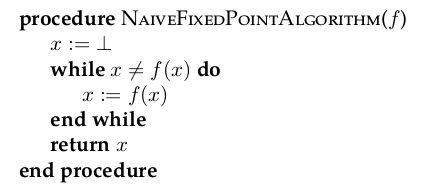
\includegraphics[width=220pt]{img/monotone/naive}
  \end{figure}
  \item A more efficient fixed-point algorithm which exploits has the structure $L^n$ and $f$ is composed from $f_1, \dots, f_n$:
  \begin{figure}[H]
  	\centering
  	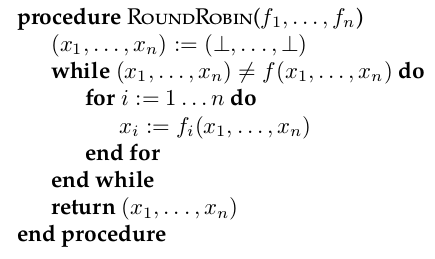
\includegraphics[width=220pt]{img/monotone/round_robin}
  \end{figure}
  \item Each iteration of the while-loop takes the same time as for the naive on but the number of iterations might be lower
  \item A more efficient algorithm is 
  \begin{figure}[H]
  	\centering
  	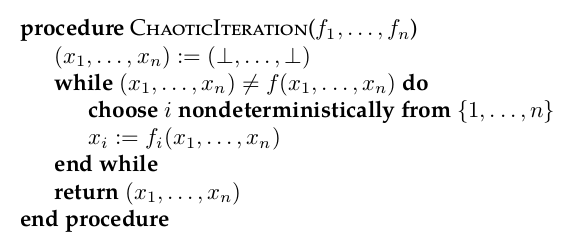
\includegraphics[width=270pt]{img/monotone/chaotic}
  \end{figure}
\end{itemize}

\subsubsection{Worklist Algorithm}
\begin{itemize}
  \item In the general case, every constraint variable $\co{v_i}$ may depend on all other variables
  \item Most often an instance of $f_i$ will only read the values of a few other variables and this can be represented as a map
  \begin{equation*}
    \text{dep} : \text{Nodes} \to 2^{\text{Nodes}}
  \end{equation*}
  it maps a node to the set of nodes whose information may depend on $v$
  \begin{itemize}
  	\item The inverse is defined as $\text{dep}^{-1}(v) = \{w \mid v \in \text{dep}(w)\}$
  	\item This is used by the following fix point algorithm
  \end{itemize}
  \begin{figure}[H]
  	\centering
  	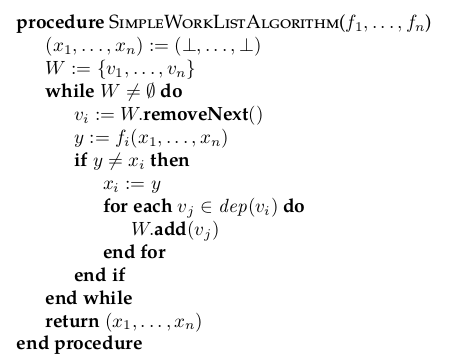
\includegraphics[width=270pt]{img/monotone/simple_worklist}
  \end{figure}
	\item Assuming that $|dep(v)|$ and $|dep^{-1}(v)|$ are bounded by a constant for all nodes $v$ the time complexity of the simple work-list algorithm can be expressed as
  \begin{equation*}
    O(n \cdot h \cdot k)
  \end{equation*}
  where $n$ is the number of CFG nodes, $h$ is the height of the lattice $L$ and $k$ is the worst-case time required to compute a constraint function $f_i(x_1, \dots, x_n)$	
\end{itemize}

\subsection{Transfer function}
\begin{itemize}
  \item All the constraints functions are on the form
  \begin{equation*}
    \co{v} = t_v(JOIN(v))
  \end{equation*}
  for some function $t_v : L \to L$ where $L$ is the lattice modeling abstract states and 
  \begin{equation*}
    JOIN(v) = \bigsqcup_{w \in dep^{-1}(v)} \co{w}
  \end{equation*}
  \item The function $t_v$ is called the \textbf{transfer function} for the CFG node $v$
  \begin{itemize}
	  \item It specifies how the analysis models the statement at $v$ as an abstract state transformer
  \end{itemize}
  \item A work-list algorithm is presented based on transfer functions that avoids some redundancy
  \begin{itemize}
  	\item The forward analysis of each variable $x_i$ denotes the abstract state for the program point before the corresponding CFG node $v_i$
  \end{itemize}
  \begin{figure}[H]
  	\centering
  	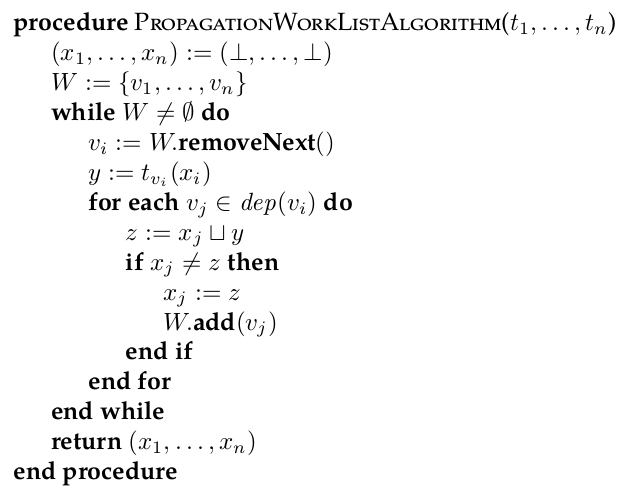
\includegraphics[width=300pt]{img/monotone/propagation}
  \end{figure}
\end{itemize}

\subsection{Widening and Narrowing}
\subsubsection{Widening}
\begin{itemize}
	\item The technique called \textbf{widening} is used in flow-sensitive analysis with infinite height lattices
  \item Let $f: L \to L$ denote the function from the fixed-point theorem and the naive fixed-point algorithm
  \item A simple form of widening, which is often sufficient, introduces a function $\omega : L \to L$ so that the sequence:
\begin{equation*}
	(\omega \circ f)^i(\bot) \text{ for } i = 0,1,\dots 
\end{equation*}
  is guaranteed to converge on a fixed point that is larger than or equal to each $f^i(\bot)$
  \begin{itemize}
	  \item To ensure that property it is sufficient that $\omega$ is monotone and extensive
	  \item Fixed point algorithms can easily be adapted to use widening by applying $\omega$ in each iteration
  \end{itemize}
  \item $\omega$ will coarse the information sufficiently to ensure termination
  \begin{itemize}
    \item Defined pointwise down to single intervals
    \item Operates relative to a fixed finite subset $B \subset N$ that must contain $- \infty$ and $\infty$
  \end{itemize}
  \item Widening generally shoots above the target
\end{itemize} 

\subsubsection{Narrowing}
\begin{itemize}
  \item Given
  \begin{align*}
    \text{fix} &= \bigsqcup f^i(\bot) \\
    \text{fix}\omega &= \bigsqcup (\omega \circ f) ^i(\bot)
  \end{align*}
The following things must be true
  \begin{itemize}
    \item $\text{fix} \sqsubseteq \text{fix}\omega$
    \item $\text{fix} \sqsubseteq f(\text{fix} \omega) \sqsubseteq \text{fix}\omega$ 
    \item Another application of $f$ may improve the result and can be iterated arbitrarily many times, which is called \textbf{Narrowing} which may improve the result
  \end{itemize}
\end{itemize}

\subsubsection{Traditional widening}
\begin{itemize}
  \item Traditional widening takes a more sophisticated approx that may lead to better analysis precision where it uses a binary operator $\nabla$
  \begin{equation*}
    \nabla : L \times L \to L
  \end{equation*}
  \item The widening operator $\nabla$ much satify
  \begin{equation*}
    \forall x,y \in L: x \sqsubseteq x \nabla y \land y \sqsubseteq x \nabla y
  \end{equation*}
  \item Using $\nabla$ a safe approximation can be given of the least fixed-point of $f$ by computing the following sequence
  \begin{align*}
    x_0 &= \bot\\
    x_{i+1} &= x_i \nabla f(x_i)
  \end{align*}
  \item This sequences eventually converges for some $k$
  \item The following is the variant of the naive fixed-point algorithm with traditional widening
  \begin{figure}[H]
  	\centering
  	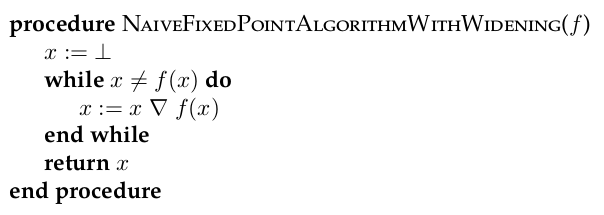
\includegraphics[width=300pt]{img/monotone/naive_widening}
  \end{figure}
\end{itemize}

\subsection{Path sensitivity}
\begin{itemize}
  \item If and while statements has been handled as a nondeterministic choice between the two branches, it is called \textbf{path insensitive} analysis
  \begin{itemize}
  	\item It fails to include some information that could potentially be used in a static analysis 
  \end{itemize}
  \item The language is extended with the artificial statement $\mathtt{assert}(E)$ where $E$ is a boolean expression to exploit the available information
  \begin{itemize}
  	\item It is inserted in places where $E$ is guaranteed to be true
  \end{itemize}
	\item Conditions on the following form $X > E$ and $E > X$ are considered which is handled by the constraint rule (interval analysis)
  \begin{equation*}
    \text{assert}(X > E): \co{v} = \text{JOIN}(v)[X \mapsto \text{gt}(\text{JOIN}(v)(X), \text{eval}(\text{JOIN}(v),E))]
  \end{equation*}
  where gt models the greater than operator:
  \begin{equation*}
    gt([l_1,h_1],[L_2,h_2]) = [l_1, h_1] \sqcup [l_2, \infty]
  \end{equation*}
  \item The use of assert statements at conditional branches provides a simple kind of path sensitivity called \textbf{control sensitivity}  
  \item A \textbf{independent attribute analyses} is where the different values of as the different values of the attributes are independent
  \item A \textbf{relational} analysis is where one keeps track of the relations between different variables
  \begin{itemize}
  	\item It can be achieved by generalizing the analysis to maintain multiple abstract states per program point
  	\item It can be done by replacing the lattice $L$ by the map lattice
  \begin{equation*}
    L^{''} = \text{Paths} \rightarrow L
  \end{equation*}
  where \textit{Paths} is a finite set of \textit{path contexts} 
  \end{itemize}
\end{itemize}

\newpage
%%% Local Variables:
%%% mode: latex
%%% TeX-master: "pav-noter"
%%% End:
